\documentclass{article}
\usepackage{amsmath, amssymb}
\usepackage{geometry}
\usepackage{tikz}
\geometry{a4paper, margin=1in}

\begin{document}

\title{Math 4580 Lecture 1: Functions and Relations}
\date{January 8, 2025}
\maketitle

\section*{Functions}
\textbf{Definition:} Let $A$ and $B$ be sets. A function $f: A \to B$ assigns exactly one output $f(a) \in B$ to every input $a \in A$. 
\begin{itemize}
    \item The set $A$ is called the \textbf{domain} of $f$.
    \item The set $B$ is called the \textbf{codomain} of $f$.
\end{itemize}

\textbf{Note:} The domain $A$, codomain $B$, and the assignment of outputs $f(a)$ to every input $a \in A$ are all part of the data defining a function. Just writing a formula like $f(x) = e^x$ does not determine a function, as the domain and codomain are not specified. For example:
\begin{itemize}
    \item $f: \mathbb{R} \to \mathbb{R}, f(x) = e^x$.
    \item $f: \mathbb{Q} \to \mathbb{Q}, f(x) = e^x$.
\end{itemize}
Although these functions use the same formula, their meanings are completely different because their domains and codomains differ.

\section*{Graphs}
A function $f: A \to B$ is often identified with its \textbf{graph} in $A \times B$:
\[ \text{graph}(f) = \{(a, b) \in A \times B : b = f(a)\}. \]

\textbf{Lemma:} Let $f: A \to B$ be a function. Its graph, $\text{graph}(f)$, passes the \textbf{vertical line test}: For every $a \in A$, $V_a := \{(a, b) \in A \times B : b \in B\}$ intersects $\text{graph}(f)$ in exactly one element.

\begin{center}
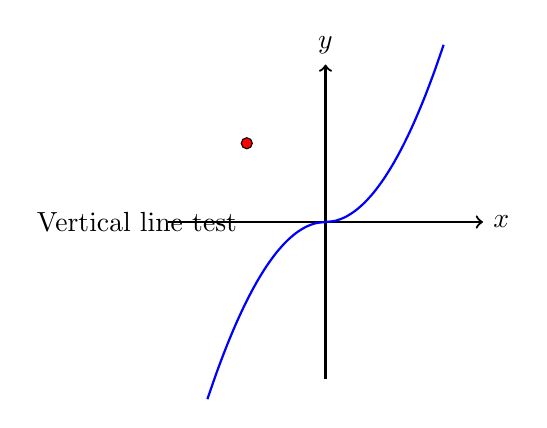
\begin{tikzpicture}
    \draw[thick,->] (-2,0) -- (2,0) node[right] {$x$};
    \draw[thick,->] (0,-2) -- (0,2) node[above] {$y$};
    \draw[domain=-1.5:1.5,smooth,variable=\x,blue,thick] plot ({\x},{\x^2});
    \draw[dashed] (-1,0) -- (-1,0) node[midway,left] {Vertical line test};
    \draw[fill=red] (-1,1) circle (2pt);
\end{tikzpicture}
\end{center}

\textbf{Proposition:} Let $G \subseteq A \times B$ be any subset passing the vertical line test, i.e., for all $a \in A$, $V_a \cap G$ consists of exactly one element. Then $G = \text{graph}(f)$ for a unique function $f: A \to B$.

\textbf{Proof:} If $G = \{(a, b) \mid b \in B\}$ satisfies the vertical line test, define $f: A \to B$ by $f(a) = b$. Then $G = \text{graph}(f)$.

\textbf{Definition:} A subset $R \subseteq A \times B$ is called a \textbf{relation}. The vertical line test distinguishes graphs of functions from more general relations.

\section*{Examples}
\begin{itemize}
    \item Let $S = \{(x, y) \in \mathbb{R}^2 : x^2 + y^2 = 1\}$ (the unit circle). This is a relation but not the graph of a function because it fails the vertical line test: The vertical line $x = 0$ intersects the circle at two points.
    \item Visual depiction of a unit circle:
    \begin{center}
    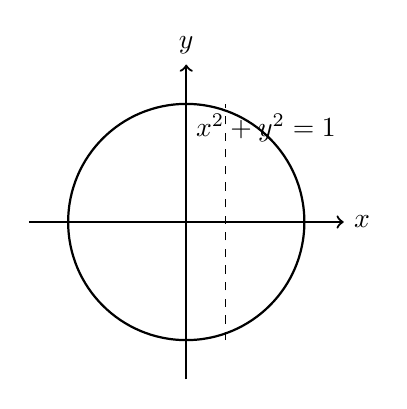
\begin{tikzpicture}
        \draw[thick,->] (-2,0) -- (2,0) node[right] {$x$};
        \draw[thick,->] (0,-2) -- (0,2) node[above] {$y$};
        \draw[thick] (0,0) circle (1.5);
        \node[below right] at (0,1.5) {$x^2 + y^2 = 1$};
        \draw[dashed] (0.5,-1.5) -- (0.5,1.5);
    \end{tikzpicture}
    \end{center}
    \item Let $A = \{1, 2, 3\}$, $B = \{4, 5\}$. The number of functions from $A$ to $B$ is $2^3 = 8$, corresponding to the $8$ associated graphs in $A \times B$.
    \item The number of relations from $A$ to $B$ is $2^{|A| \cdot |B|} = 2^{3 \cdot 2} = 64$, containing the $8$ graphs of functions from $A$ to $B$.
\end{itemize}

\textbf{Conclusion:} The notion of relation is much more permissive than the notion of functions.

\section*{Visualizing Functions as Directed Edges}
A function $f: A \to B$ can be visualized as a collection of directed edges $(a, f(a)) \in A \times B$. Each element of $A$ has exactly one outgoing edge in the graph.

\begin{center}
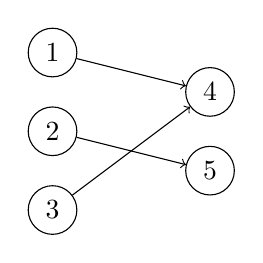
\begin{tikzpicture}
    \node[circle,draw] (A1) at (0,1) {$1$};
    \node[circle,draw] (A2) at (0,0) {$2$};
    \node[circle,draw] (A3) at (0,-1) {$3$};
    \node[circle,draw] (B1) at (2,0.5) {$4$};
    \node[circle,draw] (B2) at (2,-0.5) {$5$};
    \draw[->] (A1) -- (B1);
    \draw[->] (A2) -- (B2);
    \draw[->] (A3) -- (B1);
\end{tikzpicture}
\end{center}

\end{document}
